Ein Geiger-Müller-Zählrohr zählt allgemein die von radioaktiver Strahlung ausgelösten elektrischen Impulse.
Damit lässt sich eine Aussage über die Aktivität des Strahlers machen.
\begin{figure}[h!]
  \centering
  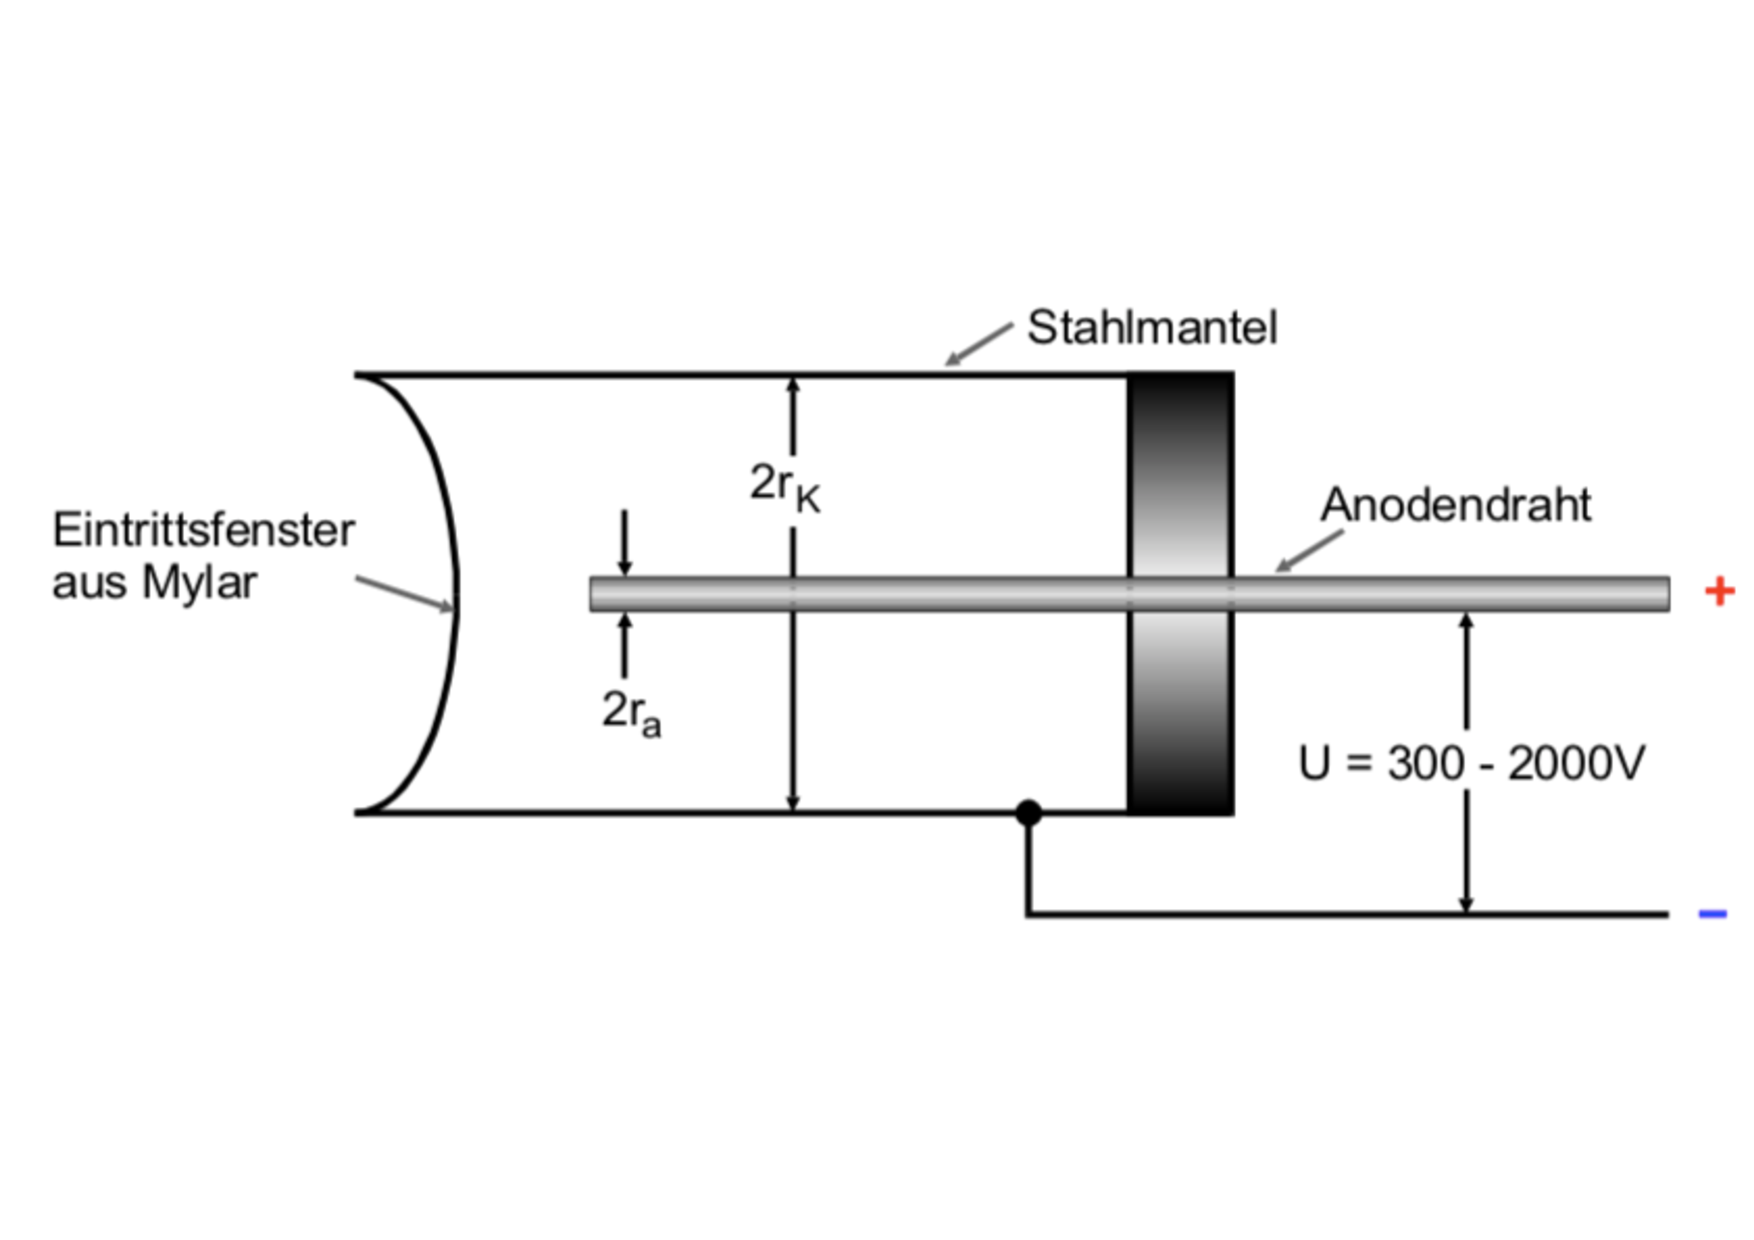
\includegraphics[width=\textwidth]{703geiger.pdf}
  \caption{Aufbau des Geiger-Müller-Zählrohrs \cite{1}}
  \label{fig:geiger}
\end{figure}
\\Ein Geiger-Müller-Zählrohr setzt sich aus einer zylinderförmigen Kathode und einem Anodendraht in der Mitte der Kathode zusammen (Abb. \ref{fig:geiger}).
Es wird eine Spannung angelegt.
Ein negativ geladenes Teilchen im Zählrohr wird also vom Anodendraht angezogen.
Der Zylinder ist dicht abgeschlossen und mit einem Gasgemisch aus Argon und Ethylalkohol gefüllt.
Eines der beiden Enden der Röhre ist mit einem Fenster versehen, das mit einer möglichst dünnen Folie ausgekleidet ist.
Ein Teilchen verliert im Zylinder nun seine Energie durch Ionisationsprozesse und trifft schließlich auf die Anode.
Somit wird ein Strom ausgelöst.
\begin{figure}[h!]
  \centering
  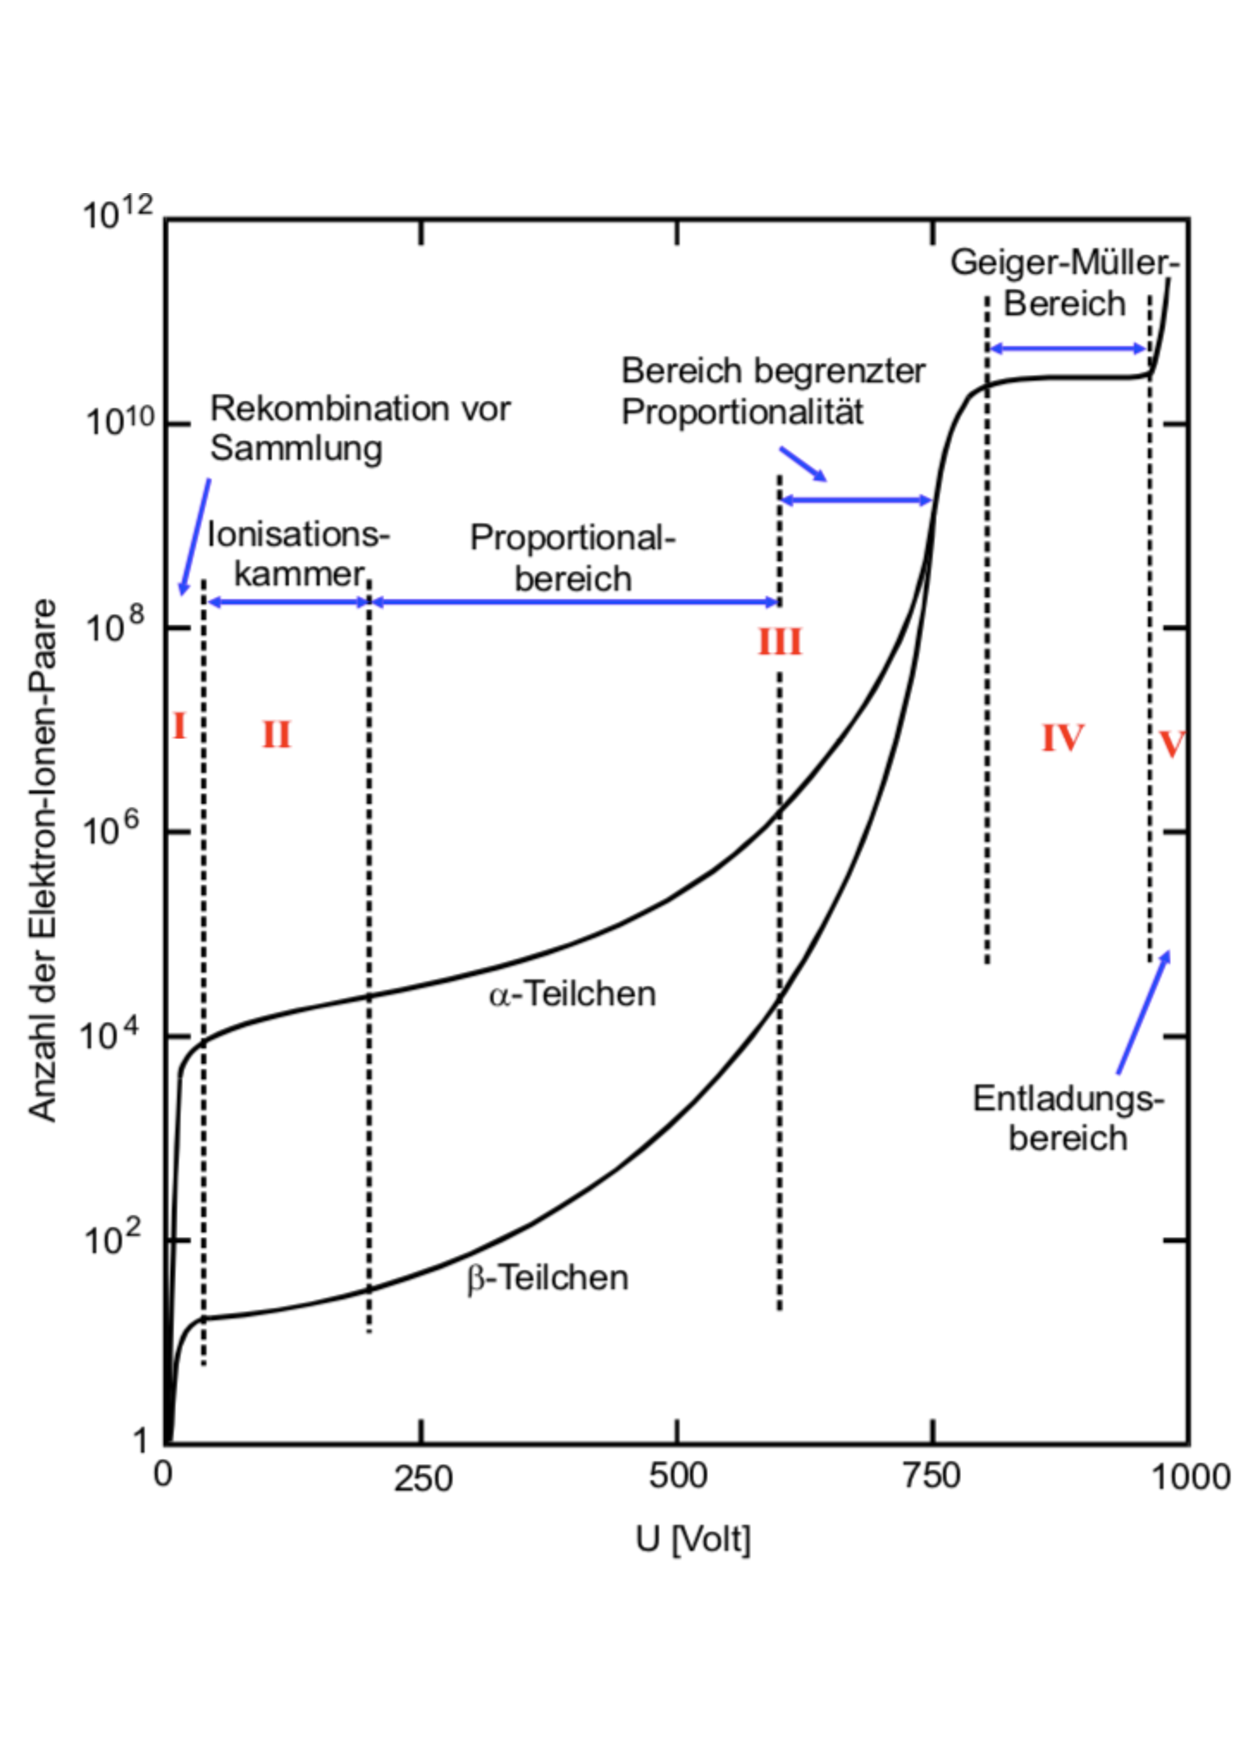
\includegraphics[width=\textwidth]{703charakteristik.pdf}
  \caption{Zählrate gegen die angelegte Spannung am Geiger-Müller-Zählrohr \cite{1}}
  \label{fig:charakteristik}
\end{figure}
\\Wird die Zählrate gegen die angelegte Spannung aufgetragen, lässt sich der Verlauf in verschiedene Abschnitte einteilen (Abb. \ref{fig:charakteristik}).
\\Im Bereich der Rekombination werden zwar Atome ionisiert, doch die ausgelösten Elektronen werden direkt wieder von den Atomen absorbiert.
So kann hier keine Zählrate gemessen werden.
\\Das Zählrohr kann auch als Ionisationskammer bezeichnet werden, solange die Zählrate abhängig von der Energie und Intensität der Strahlung ist.
\\Höhere Spannungen sorgen dafür, dass die ausgeschlagenen Elektronen unterwegs zu der Anode weitere Atome ionisieren.
Die Zahl dieser Elektronen steigt lawinenartig an (Townsend-Lawine).
Der Bereich wird Proportionalzählrohr genannt.
\\Wird die Spannung noch größer, wird der sogenannte Auslösebereich erreicht.
Dabei ionisieren die eindringenden Teilchen erst einzelne Gasatome.
Die gelösten Elektronen haben genug Energie um weitere Atome zu ionisieren.
Bei der Ionisation entstehen auch Photonen mit genug Energie um weitere Atome zu ionisieren.
Die Photonen sind ungeladen und bewegen sich unabhängig vom elektrischen Feld im Zählrohr.
Dieses Phänomen läuft nun lawinenartig durch das gesamte Zählrohr.
Die Messung der Energie der Teilchen ist nun nicht mehr möglich, da die Ladung unabhänigig von der Primärionisation ist.
In diesem Bereich ist der übliche Messbereich des Geiger-Müller-Zählrohrs.
\\Bei der Untersuchung des Geiger-Müller-Zählrohrs sind weitere besondere Effekte zu beobachten.
\begin{figure}[h!]
  \centering
  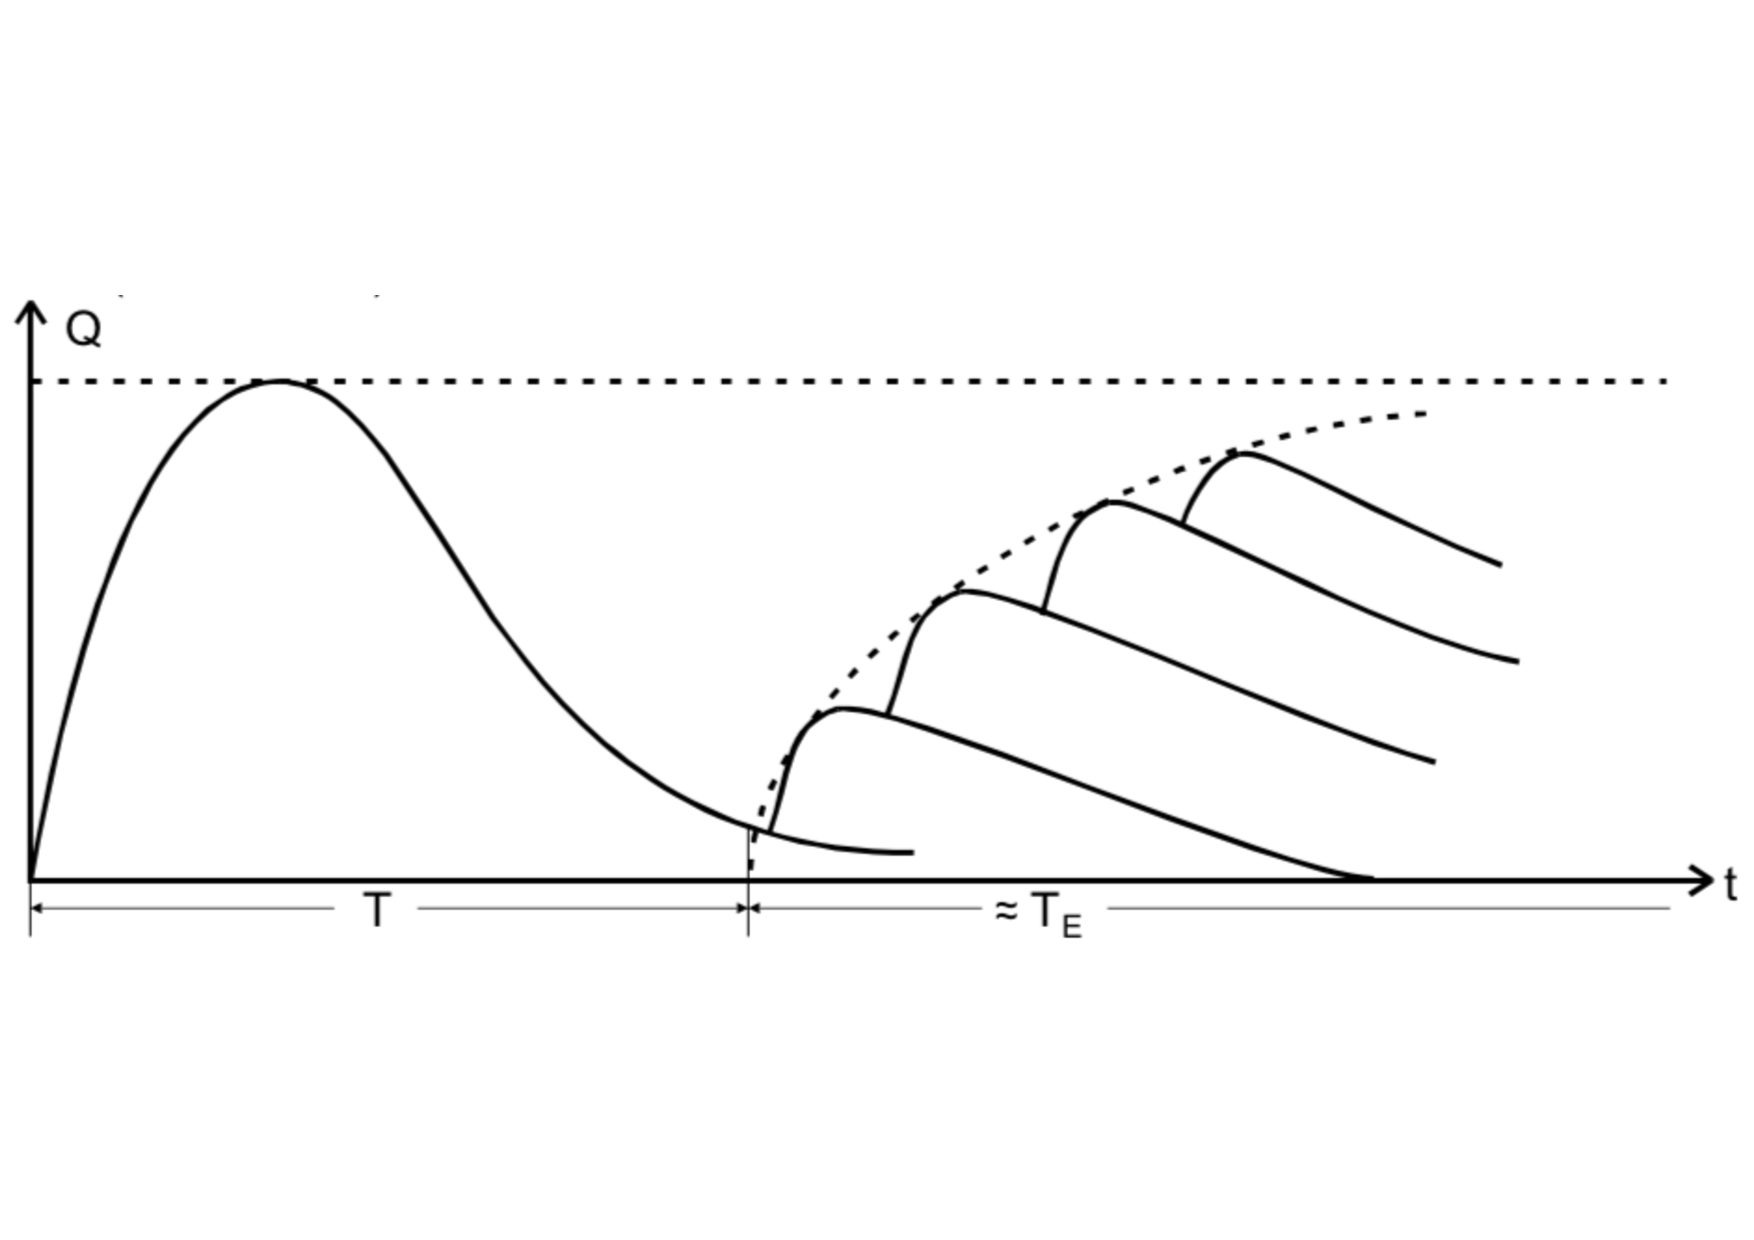
\includegraphics[width=\textwidth]{703totzeit.pdf}
  \caption{Ladung gegen die Zeit mit markierter Totzeit $T$ und Erholungszeit $T_{E}$ \cite{1}}
  \label{fig:totzeit}
\end{figure}
\\Als Totzeit $T$ wird die Zeit nach einem ausgelösten Impuls bezeichnet, in der kein weiterer Impuls ausgelöst werden kann (Abb. \ref{fig:totzeit}).
Entsprechend werden im Bereich der Totzeit die eintreffenden Teilchen nicht gezählt.
Dies entsteht durch die langsamen und schweren Ionen, die bei der Ionisation entstehen.
Die Ionenwolken verändern kurzfristig und lokal die Raumladung.
Die Totzeit lässt sich an einem angeschlossen Oszilloskop ablesen oder über zwei verschiedene Strahlungsquellen messen.
Letztere Methode funktioniert über den Unterschied zwischen der gemessenen Zählrate $N_{R}$ und der tatsächlichen Zählrate $N_{W}$.
Die wahre Zählrate $N_{W}$ berechnet sich über
\begin{align*}
  N_{W}=\frac{N_{R}}{1-T \cdot N_{R}}.
\end{align*}
Hiermit lässt sich die Totzeit bestimmen.
Dazu werden für zwei verschiedene Strahler und die Kombination der beiden Strahlungsquellen die registrierte Zählrate $N_{R}$ ausgemessen.
Damit berechnen sich die jeweiligen wahren Zählraten $N_{W}$:
\begin{align*}
  N_{W, 1}& =\frac{N_{R_{1}}}{1-T \cdot N_{R_{1}}}\\
  N_{W, 2}& =\frac{N_{R_{2}}}{1-T \cdot N_{R_{2}}}\\
  N_{W, 1+2}& =\frac{N_{R_{1+2}}}{1-T \cdot N_{R_{1+2}}}.
\end{align*}
Mit der Näherung $T^2 N_{R}^2 \ll 1$ ergibt sich
\begin{align}
  T \approx \frac{N_{R_{1}}+N_{R_{2}}-N_{R_{1+2}}}{2 N_{R_{1}} N_{R_{2}}}.
  \label{eqn:T}
\end{align}
\\Die Ionenwolken lösen sich langsam auf und sorgen auch bei den nächsten Impulsauslösungen für eine abgeschwächte Spannung.
Die sogenannte Erholungszeit $T_{E}$ ist die Zeit, die vergeht, bis die Impulse wieder die ursprüngliche Höhe haben.
\\Ein weiteres Phänomen sind die Nachentladungen.
Die Elektronen im Zählrohr können aus dem Kathodenmaterial Elektronen ausschlagen.
Diese "Sekundärelektronen" können ihrerseits wieder Entladungen auslösen.
Dies wird dann Nachentladung genannt.
Zur Vermeidung der Nachentladungen ist in dem Gas Alkohol beigemischt.
Die Alkoholmoleküle absorbieren die Energie der Photonen, indem sie sie in Schwingungen verwandelt.
\begin{figure}[h!]
  \centering
  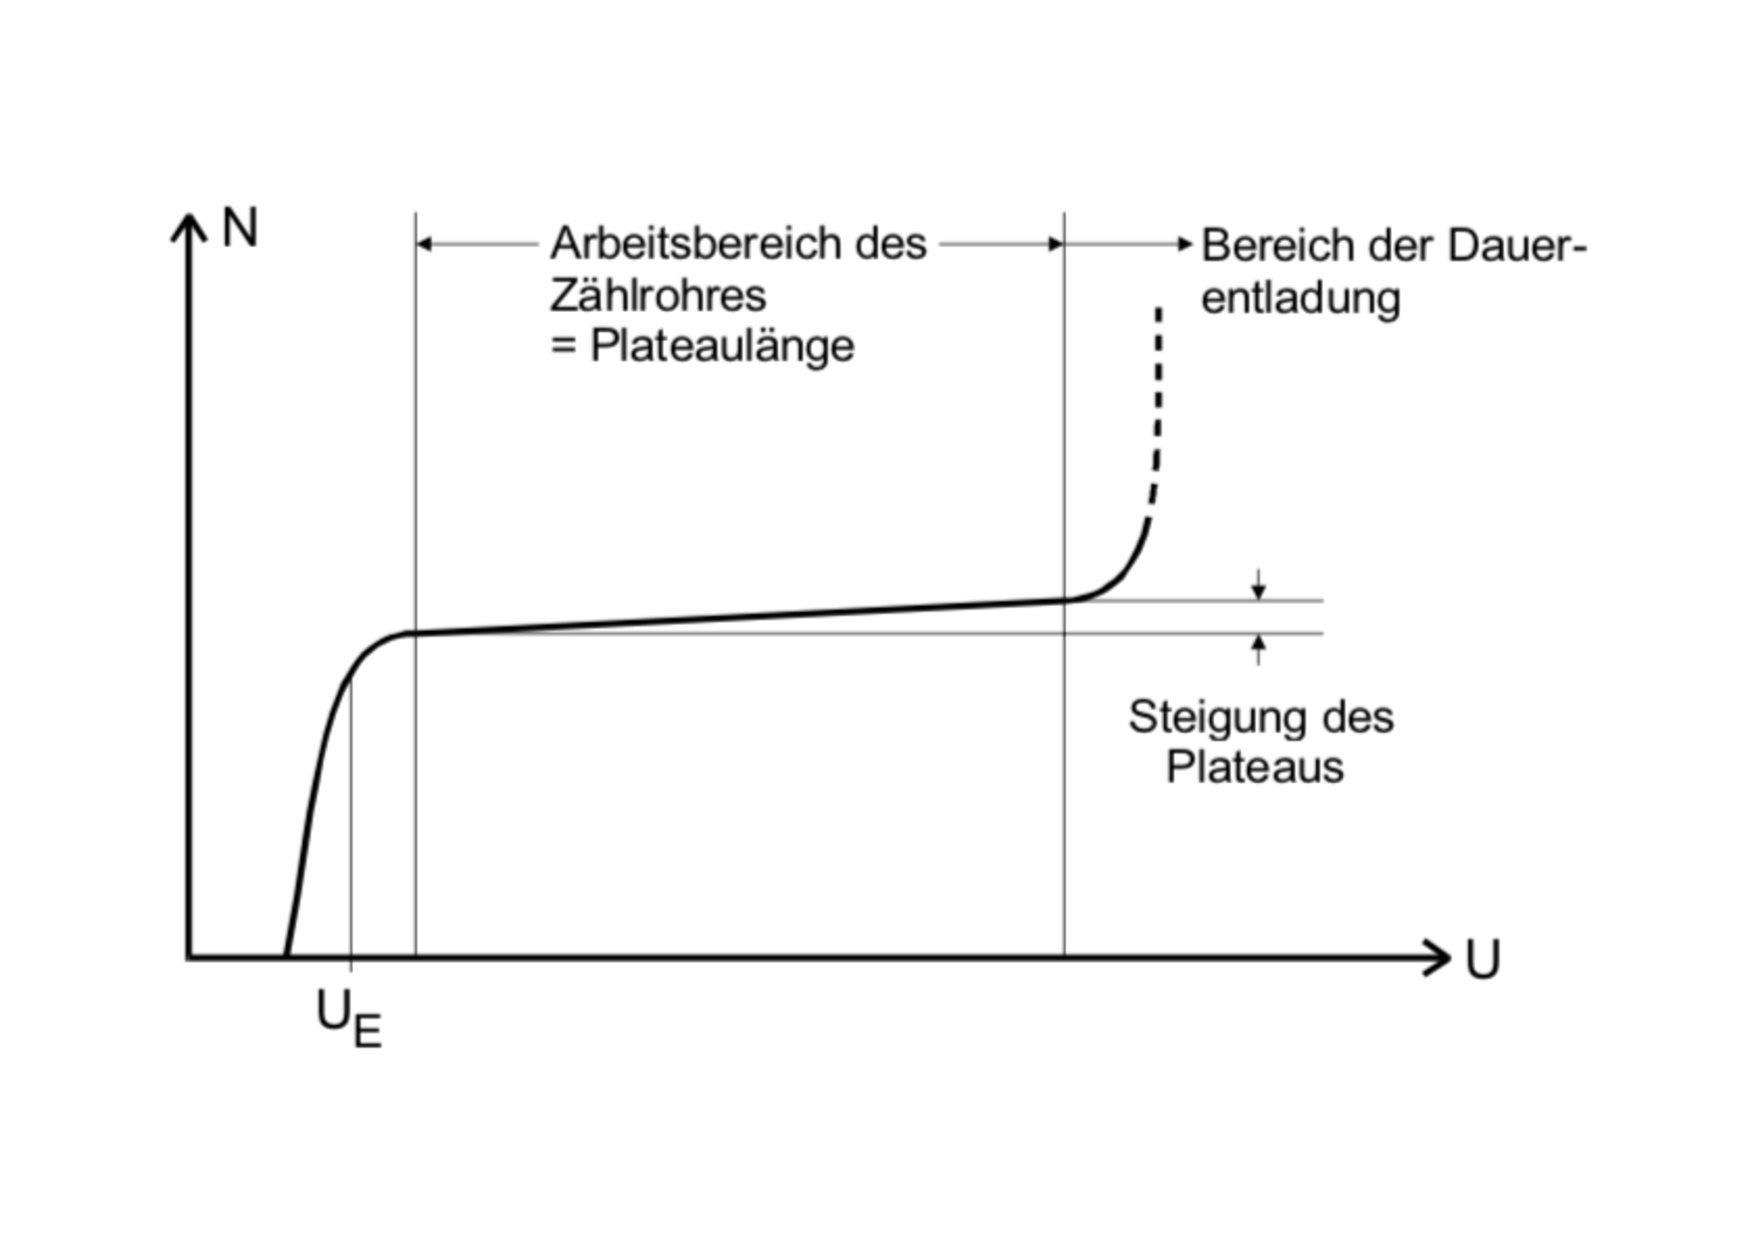
\includegraphics[width=\textwidth]{703plateau.pdf}
  \caption{Ladung gegen die Zeit mit markiertem Plateau \cite{1}}
  \label{fig:plateau}
\end{figure}
\\Die Charakteristik eines Geiger-Müller-Zählrohrs hat ein auffälliges Plateau (Abb.\ref{fig:plateau}).
Idealerweise ist die Steigung im Plateau null, aber dies ist durch den unumgänglichen Rest der Nachentladungen nicht vermeidbar.
\\Bei großen Zählraten entsteht ein messbarer Strom in der Anode.
Der Strom lässt sich durch
\begin{align}
  I= \frac{\Delta Q}{\Delta t}Z \leftrightarrow \Delta Q = \frac{I \Delta t}{Z}
  \label{eqn:I}
\end{align}
berechnen.
Dabei ist $Z$ die Anzahl der gemessenen Teilchen, $Q$ die Ladung und $t$ die Zeit.
\\Wird die Spannung noch größer, kann das Gas in der Röhre sich selbst entladen und das Zählrohr kann kaputt gehen.
\\In dem Geiger-Müller-Zählrohr können hauptsächlich $\alpha$- und $\beta$-Strahlung nachgewiesen werden.
Die $\gamma$-Quanten haben als Initialerreger kaum Auswirkungen auf das Zählrohr.



\FloatBarrier
